%!TEX root = ../thesis.tex

\section{Convolution Neural Network}
畳み込みニューラルネットワーク(convolutional neural network:CNN)は人工ニューラルネットワークのモデルの一種である. このモデルは, 画像や音声などの多次元の配列で表される複雑なデータを処理するために特別に設計されている. CNNは次のような特徴を持つ層で構成されている.
\begin{enumerate}
  \item 畳み込み層\\入力データをフィルタ(カーネル)を用いて特徴を抽出する.
  \item プーリング層\\特徴を残しつつ, 畳み込み層の出力を圧縮する. これにより, 画像であればピクセル数が減少し, 計算量を大幅に減らすことができる.
  \item 全結合層\\畳み込み層とプーリング層の出力をまとめて処理する.
\end{enumerate}

Krizhevskyら\cite{AlexNet}は\figref{Fig:AlexNet}で示すような, 8層のネットワークを用いて, 画像分類タスクをエラー率15.3\%で達成し, 画像分類コンペティションである ILSVRC(ImageNet Large Scale VisualRecognition Competition)2012で優勝した.

\vspace{0.5cm}

\begin{figure}[hbtp]
  \centering
 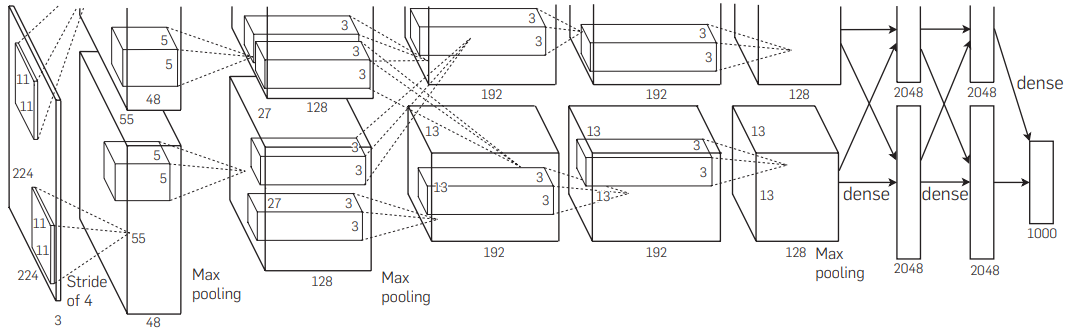
\includegraphics[keepaspectratio, scale=0.35]
      {images/Alexnet.png}
 \caption{AlexNet from \cite{AlexNet}}
 \label{Fig:AlexNet}
\end{figure}
\newpage
Simonyan\cite{simonyan}らはCNNの層の深さが精度に与える影響を調査した. \figref{Fig:VGG}のような, 最大19層の深い畳み込みネットワークを評価した. その結果, モデルを深層にすることが分類精度に有利であることが示された.
ILSVRC2012の優勝モデルであるAlexNetは8層, ILSVRC2013で提案されたZFNetは同様の8層であることから, 当時のCNNとしては圧倒的に深い層を持つモデルであった. このような深い畳み込みネットワークは, 深層学習における重要な発展の一つとされている.
\begin{figure}[hbtp]
  \centering
 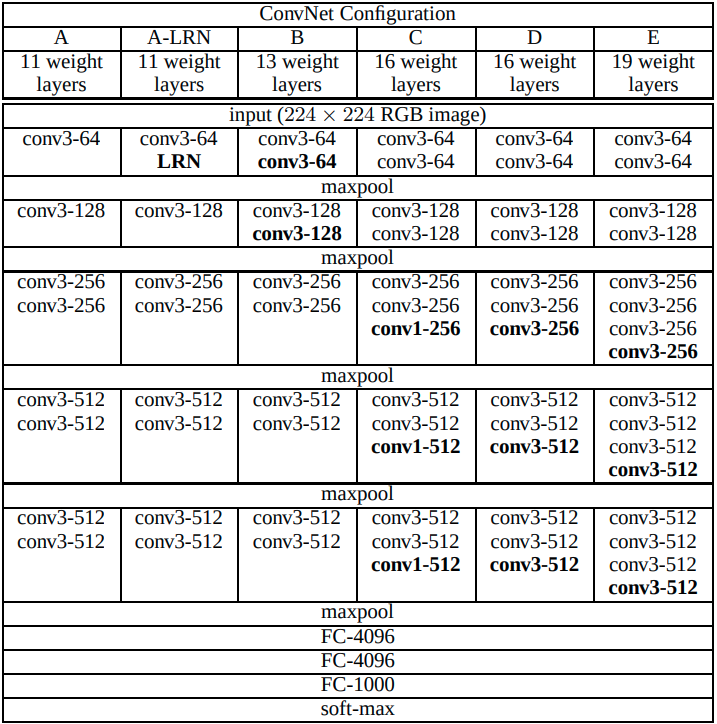
\includegraphics[keepaspectratio, scale=0.5]
      {images/VGG2.png}
 \caption{VGG from \cite{AlexNet}}
 \label{Fig:VGG}
\end{figure}


% \vspace{5cm}

% \begin{figure}[hbtp]
%   \centering
%  \includegraphics[keepaspectratio, scale=0.7]
%       {images/end-to-end.png}
%  \caption{Structure of end-to-end learning}
%  \label{Fig:end-to-end}
% \end{figure}

% \subsubsection{etc...}
\newpage
